\documentclass[11pt,a4paper]{report}
\usepackage[textwidth=37em,vmargin=30mm]{geometry}
\usepackage{calc,xunicode,amsmath,amssymb,paralist,enumitem,tabu,booktabs,datetime2,xeCJK,xeCJKfntef,listings}
\usepackage{tocloft,fancyhdr,tcolorbox,xcolor,graphicx,eso-pic,xltxtra,xelatexemoji}

\newcommand{\envyear}[0]{2025}
\newcommand{\envdatestr}[0]{2025-04-15}
\newcommand{\envfinaldir}[0]{webdb/2025/20250415/final}

\usepackage[hidelinks]{hyperref}
\hypersetup{
    colorlinks=false,
    pdfpagemode=FullScreen,
    pdftitle={Web Digest - \envdatestr}
}

\setlength{\cftbeforechapskip}{10pt}
\renewcommand{\cftchapfont}{\rmfamily\bfseries\large\raggedright}
\setlength{\cftbeforesecskip}{2pt}
\renewcommand{\cftsecfont}{\sffamily\small\raggedright}

\setdefaultleftmargin{2em}{2em}{1em}{1em}{1em}{1em}

\usepackage{xeCJK,xeCJKfntef}
\xeCJKsetup{PunctStyle=plain,RubberPunctSkip=false,CJKglue=\strut\hskip 0pt plus 0.1em minus 0.05em,CJKecglue=\strut\hskip 0.22em plus 0.2em}
\XeTeXlinebreaklocale "zh"
\XeTeXlinebreakskip = 0pt


\setmainfont{Brygada 1918}
\setromanfont{Brygada 1918}
\setsansfont{IBM Plex Sans}
\setmonofont{JetBrains Mono NL}
\setCJKmainfont{Noto Serif CJK SC}
\setCJKromanfont{Noto Serif CJK SC}
\setCJKsansfont{Noto Sans CJK SC}
\setCJKmonofont{Noto Sans CJK SC}

\setlength{\parindent}{0pt}
\setlength{\parskip}{8pt}
\linespread{1.15}

\lstset{
	basicstyle=\ttfamily\footnotesize,
	numbersep=5pt,
	backgroundcolor=\color{black!5},
	showspaces=false,
	showstringspaces=false,
	showtabs=false,
	tabsize=2,
	captionpos=b,
	breaklines=true,
	breakatwhitespace=true,
	breakautoindent=true,
	linewidth=\textwidth
}






\newcommand{\coverpic}[2]{
    % argv: itemurl, authorname
    Cover photo by #2~~(\href{#1}{#1})
}
\newcommand{\makeheader}[0]{
    \begin{titlepage}
        % \newgeometry{hmargin=15mm,tmargin=21mm,bmargin=12mm}
        \begin{center}
            
            \rmfamily\scshape
            \fontspec{BaskervilleF}
            \fontspec{Old Standard}
            \fontsize{59pt}{70pt}\selectfont
            WEB\hfill DIGEST
            
            \vfill
            % \vskip 30pt
            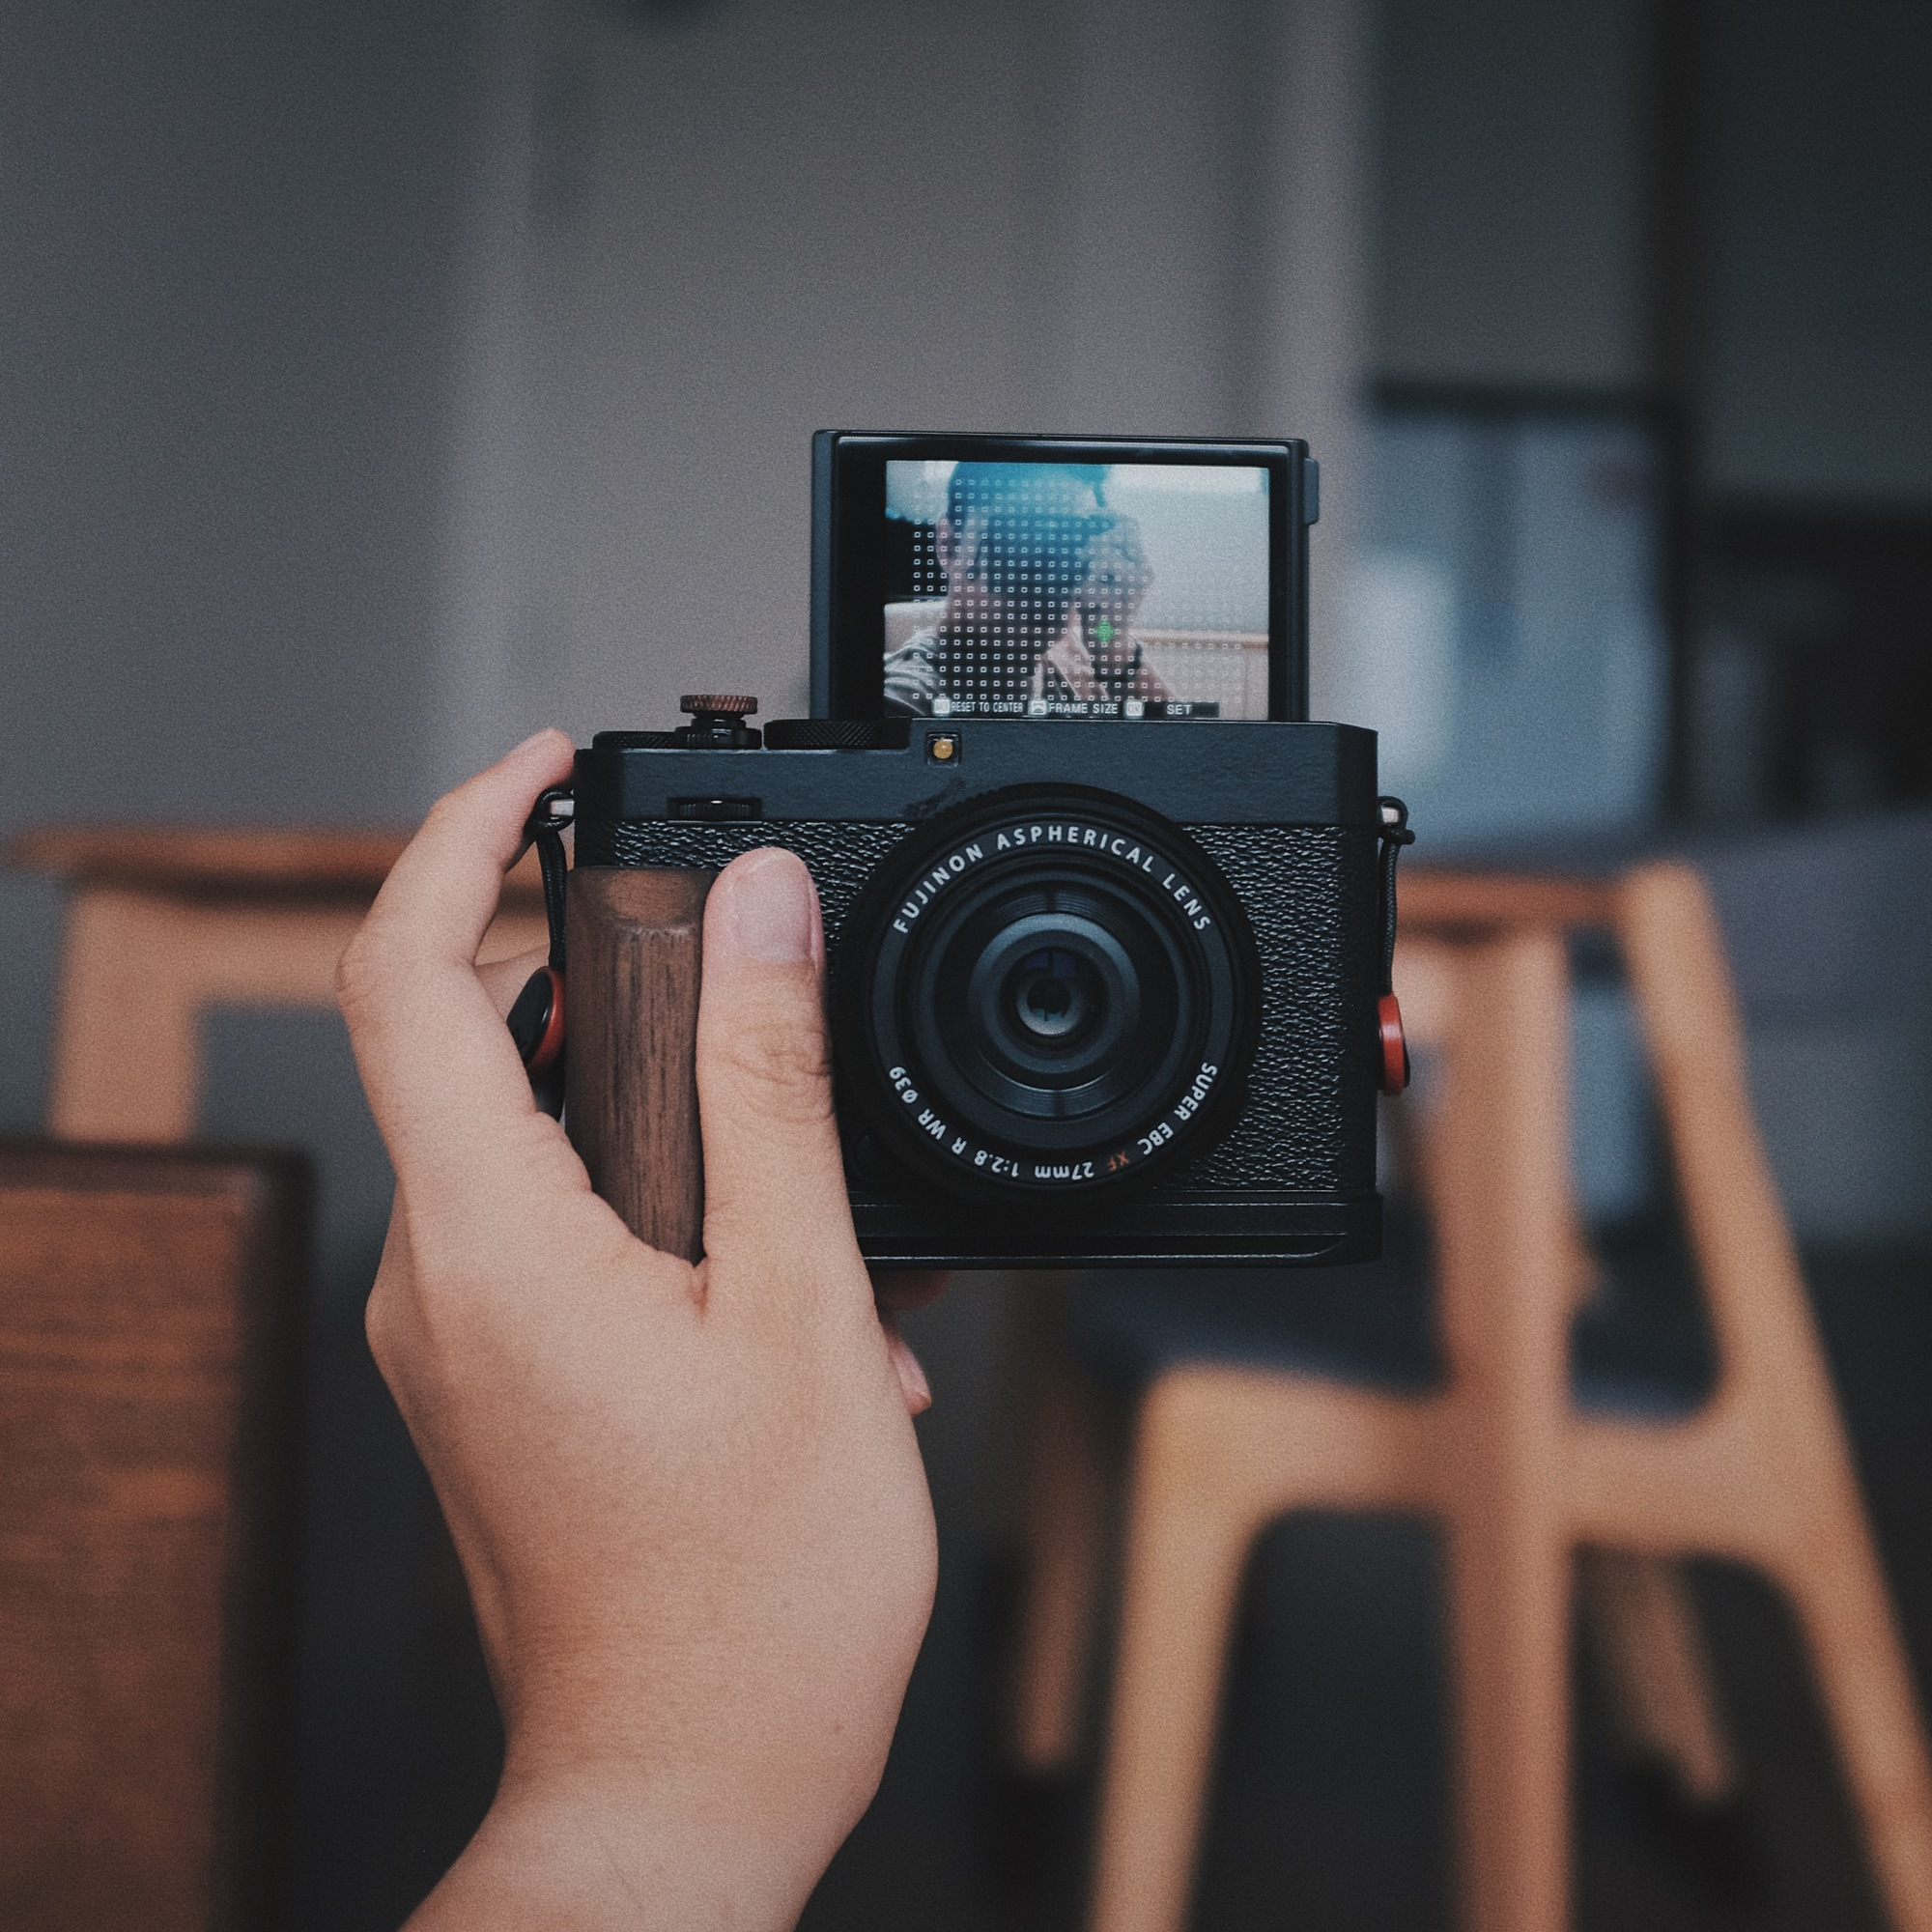
\includegraphics[width=\linewidth]{\envfinaldir/coverpic-prod.jpg}\par
            % \vskip 30pt
            \vfill

            \normalsize\rmfamily\scshape
            \copyright{} The Web Digest Project \hfill\large \envdatestr
        \end{center}
    \end{titlepage}
    % \restoregeometry
}
\newcommand{\simplehref}[1]{%
    \textcolor{blue!80!green}{\href{#1}{#1}}%
}
\renewcommand{\contentsname}{\center\Huge\sffamily\bfseries Contents\par\vskip 20pt}
\newcounter{ipartcounter}
\setcounter{ipartcounter}{0}
\newcommand{\ipart}[1]{
    % \vskip 20pt
    \clearpage
    \stepcounter{ipartcounter}
    \phantomsection
    \addcontentsline{toc}{chapter}{#1}
    % \begin{center}
    %     \Huge
    %     \sffamily\bfseries
    %     #1
    % \end{center}
    % \vskip 20pt plus 7pt
}
\newcounter{ichaptercounter}
\setcounter{ichaptercounter}{0}
\newcommand{\ichapter}[1]{
    % \vskip 20pt
    \clearpage
    \stepcounter{ichaptercounter}
    \phantomsection
    \addcontentsline{toc}{section}{\numberline{\arabic{ichaptercounter}}#1}
    \begin{center}
        \Huge
        \sffamily\bfseries
        #1
    \end{center}
    \vskip 20pt plus 7pt
}
\newcommand{\entrytitlefont}[1]{\subsection*{\raggedright\Large\sffamily\bfseries#1}}
\newcommand{\entryitemGeneric}[2]{
    % argv: title, url
    \parbox{\linewidth}{
        \entrytitlefont{#1}\par\vskip 5pt
        \footnotesize\ttfamily\mdseries
        \simplehref{#2}
    }\vskip 11pt plus 11pt minus 1pt
}
\newcommand{\entryitemGithub}[3]{
    % argv: title, url, desc
    \parbox{\linewidth}{
        \entrytitlefont{#1}\par\vskip 5pt
        \footnotesize\ttfamily\mdseries
        \simplehref{#2}\par\vskip 5pt
        \small\rmfamily\mdseries#3
    }\vskip 11pt plus 11pt minus 1pt
}
\newcommand{\entryitemAp}[3]{
    % argv: title, url, desc
    \parbox{\linewidth}{
        \entrytitlefont{#1}\par\vskip 5pt
        \footnotesize\ttfamily\mdseries
        \simplehref{#2}\par\vskip 5pt
        \small\rmfamily\mdseries#3
    }\vskip 11pt plus 11pt minus 1pt
}
\newcommand{\entryitemHackernews}[3]{
    % argv: title, hnurl, rawurl
    % \parbox{\linewidth}{
    %     \entrytitlefont{#1}\par\vskip 5pt
    %     \footnotesize\ttfamily\mdseries
    %     \simplehref{#3}\par
    %     \textcolor{black!50}{\href{#2}{#2}}
    % }\vskip 11pt plus 11pt minus 1pt
    \begin{minipage}{\linewidth}
            \entrytitlefont{#1}\par\vskip 5pt
            \footnotesize\ttfamily\mdseries
            \simplehref{#3}\par
            \textcolor{black!50}{\href{#2}{#2}}
    \end{minipage}\par\vskip 11pt plus 11pt minus 1pt
}







\begin{document}

\makeheader

\tableofcontents\clearpage




\ipart{Developers}
\ichapter{Hacker News}
\entryitemTwoLinks{Intel sells 51\% stake in Altera to private equity firm on a \$8.75B valuation}{https://news.ycombinator.com/item?id=43686773}{https://newsroom.intel.com/corporate/intel-partner-deal-news-april2025}

\entryitemTwoLinks{What Is Entropy?}{https://news.ycombinator.com/item?id=43684560}{https://jasonfantl.com/posts/What-is-Entropy/}

\entryitemTwoLinks{Harvard's response to federal government letter demanding changes}{https://news.ycombinator.com/item?id=43684536}{https://www.harvard.edu/president/news/2025/the-promise-of-american-higher-education/}

\entryitemTwoLinks{Federal Government's letter to Harvard demanding changes [pdf]}{https://news.ycombinator.com/item?id=43684386}{https://www.harvard.edu/research-funding/wp-content/uploads/sites/16/2025/04/Letter-Sent-to-Harvard-2025-04-11.pdf}

\entryitemTwoLinks{GPT-4.1 in the API}{https://news.ycombinator.com/item?id=43683410}{https://openai.com/index/gpt-4-1/}

\entryitemTwoLinks{U.S. and El Salvador Say They Won't Return Man Who Was Mistakenly Deported}{https://news.ycombinator.com/item?id=43683405}{https://www.nytimes.com/live/2025/04/14/us/trump-news-tariffs}

\entryitemTwoLinks{OpenAI Is a Systemic Risk to the Tech Industry}{https://news.ycombinator.com/item?id=43683071}{https://www.wheresyoured.at/openai-is-a-systemic-risk-to-the-tech-industry-2/}

\entryitemTwoLinks{The path to open-sourcing the DeepSeek inference engine}{https://news.ycombinator.com/item?id=43682088}{https://github.com/deepseek-ai/open-infra-index/tree/main/OpenSourcing\_DeepSeek\_Inference\_Engine}

\entryitemTwoLinks{SQLite File Format Viewer}{https://news.ycombinator.com/item?id=43682006}{https://sqlite-internal.pages.dev}

\entryitemTwoLinks{How to Bike Across the Country}{https://news.ycombinator.com/item?id=43681936}{https://www.brooks.team/posts/how-to-bike-across-the-country/}

\entryitemTwoLinks{A hackable AI assistant using a single SQLite table and a handful of cron jobs}{https://news.ycombinator.com/item?id=43681287}{https://www.geoffreylitt.com/2025/04/12/how-i-made-a-useful-ai-assistant-with-one-sqlite-table-and-a-handful-of-cron-jobs}

\entryitemTwoLinks{Meta antitrust trial kicks off in federal court}{https://news.ycombinator.com/item?id=43680957}{https://www.axios.com/pro/tech-policy/2025/04/14/ftc-meta-antitrust-trial-kicks-off-in-federal-court}

\entryitemTwoLinks{DolphinGemma: How Google AI is helping decode dolphin communication}{https://news.ycombinator.com/item?id=43680899}{https://blog.google/technology/ai/dolphingemma/}

\entryitemTwoLinks{Meilisearch – search engine API bringing AI-powered hybrid search}{https://news.ycombinator.com/item?id=43680699}{https://github.com/meilisearch/meilisearch}

\entryitemTwoLinks{Omnom: Self-hosted bookmarking with searchable, wysiwyg snapshots [showcase]}{https://news.ycombinator.com/item?id=43680232}{https://omnom.zone/?src=hn}

\entryitemTwoLinks{Hacktical C: practical hacker's guide to the C programming language}{https://news.ycombinator.com/item?id=43679781}{https://github.com/codr7/hacktical-c}

\entryitemTwoLinks{Zig's new LinkedList API (it's time to learn fieldParentPtr)}{https://news.ycombinator.com/item?id=43679707}{https://www.openmymind.net/Zigs-New-LinkedList-API/}

\entryitemTwoLinks{Kezurou-Kai \#39}{https://news.ycombinator.com/item?id=43679004}{https://www.bigsandwoodworking.com/kezurou-kai-39/}

\entryitemTwoLinks{Albert Einstein's theory of relativity in words of four letters or less (1999)}{https://news.ycombinator.com/item?id=43678312}{https://www.muppetlabs.com/~breadbox/txt/al.html}

\entryitemTwoLinks{Mario Vargas Llosa has died}{https://news.ycombinator.com/item?id=43677917}{https://www.nytimes.com/2025/04/13/books/review/mario-vargas-llosa-appraisal.html}\ichapter{Phoronix}
\entryitemGeneric{\hskip 0pt{}GNOME Shell Frippery Makes It Into Debian Unstable For A GNOME2-Like Experience}{https://www.phoronix.com/news/GNOME-Shell-Frippery-Debian}

\entryitemGeneric{\hskip 0pt{}Manjaro Summit Now In Alpha For Semi-Immutable, Atomically Updated Arch Linux Distro}{https://www.phoronix.com/news/Manjaro-Summit-Alpha}

\entryitemGeneric{\hskip 0pt{}Intel Engineer Preparing To Land Change For Cleaning Up 32-bit x86 Linux Kernel Code}{https://www.phoronix.com/news/Linux-Nears-32bit-PTI-PAE-Unify}

\entryitemGeneric{\hskip 0pt{}Intel Lunar Lake On Linux Can Roughly Match Windows 11 Xe2 Graphics - When Not Stuck At 400MHz}{https://www.phoronix.com/review/lunarlake-xe2-windows-linux-2025}

\entryitemGeneric{\hskip 0pt{}Kexec HandOver "KHO" Looks Like It Might Be Ready For The Linux 6.16 Kernel}{https://www.phoronix.com/news/Kexec-HandOver-KHO-Linux-MM}

\entryitemGeneric{\hskip 0pt{}Intel Sells 51\% Of Its Altera Business}{https://www.phoronix.com/news/Intel-Sells-51p-Altera}

\entryitemGeneric{\hskip 0pt{}Intel Begins Linux Preparations For Bartlett Lake}{https://www.phoronix.com/news/Intel-Bartlett-Lake-Linux-Start}

\entryitemGeneric{\hskip 0pt{}AMD RDNA4 Paired Context Reg Feature Merged For RADV To Potentially Help Performance}{https://www.phoronix.com/news/AMD-RDNA4-Paired-Context-Regs}

\entryitemGeneric{\hskip 0pt{}Linux PCACHE Proposed For Persistent Memory Cache For Block Devices}{https://www.phoronix.com/news/Linux-PCACHE-RFC}\ichapter{Dribbble}
\entryitemGeneric{\hskip 0pt{}Lion sketches}{https://dribbble.com/shots/25898381-Lion-sketches}

\entryitemGeneric{\hskip 0pt{}Chat App - Two Pages of Sketches}{https://dribbble.com/shots/25890352-Chat-App-Two-Pages-of-Sketches}

\entryitemGeneric{\hskip 0pt{}Nite Riot®\_Film Production // Case Study\_Vol.2.0}{https://dribbble.com/shots/25889874-Nite-Riot-Film-Production-Case-Study-Vol-2-0}

\entryitemGeneric{\hskip 0pt{}Lock Layer Logo Design - Shield, Letter L, Cube, Security}{https://dribbble.com/shots/25889313-Lock-Layer-Logo-Design-Shield-Letter-L-Cube-Security}

\entryitemGeneric{\hskip 0pt{}🔐 Cybersecurity Mobile App}{https://dribbble.com/shots/25887711--Cybersecurity-Mobile-App}

\entryitemGeneric{\hskip 0pt{}Lion}{https://dribbble.com/shots/25884438-Lion}

\entryitemGeneric{\hskip 0pt{}Hollo Logo Design}{https://dribbble.com/shots/25883411-Hollo-Logo-Design}

\entryitemGeneric{\hskip 0pt{}Adobe Acrobat Logo Redesign Concept}{https://dribbble.com/shots/25884888-Adobe-Acrobat-Logo-Redesign-Concept}

\entryitemGeneric{\hskip 0pt{}Corti: Visual identity exploration}{https://dribbble.com/shots/25871312-Corti-Visual-identity-exploration}

\entryitemGeneric{\hskip 0pt{}Fintech Web Design \& Landing Page for Puzzle}{https://dribbble.com/shots/25652139-Fintech-Web-Design-Landing-Page-for-Puzzle}

\entryitemGeneric{\hskip 0pt{}Web Design Crypto Trading}{https://dribbble.com/shots/25879747-Web-Design-Crypto-Trading}

\entryitemGeneric{\hskip 0pt{}Monster Pony Wooden toy}{https://dribbble.com/shots/25880300-Monster-Pony-Wooden-toy}

\entryitemGeneric{\hskip 0pt{}Educate AI Logo Design - Letter E, Monogram, Education}{https://dribbble.com/shots/25879659-Educate-AI-Logo-Design-Letter-E-Monogram-Education}

\entryitemGeneric{\hskip 0pt{}Polydex}{https://dribbble.com/shots/25879909-Polydex}

\entryitemGeneric{\hskip 0pt{}Greetings from}{https://dribbble.com/shots/25881723-Greetings-from}

\entryitemGeneric{\hskip 0pt{}Kilo Code - Branding}{https://dribbble.com/shots/25881666-Kilo-Code-Branding}

\entryitemGeneric{\hskip 0pt{}Hawkridge}{https://dribbble.com/shots/25877367-Hawkridge}

\entryitemGeneric{\hskip 0pt{}UI Design for Cargo Delivery Company}{https://dribbble.com/shots/25874804-UI-Design-for-Cargo-Delivery-Company}

\entryitemGeneric{\hskip 0pt{}Nite Riot®\_Film Production // Case Study\_Vol.1.0}{https://dribbble.com/shots/25874978-Nite-Riot-Film-Production-Case-Study-Vol-1-0}

\entryitemGeneric{\hskip 0pt{}UltraSlot}{https://dribbble.com/shots/25875506-UltraSlot}

\entryitemGeneric{\hskip 0pt{}Sidekick Ai 3d mascot}{https://dribbble.com/shots/25874949-Sidekick-Ai-3d-mascot}

\entryitemGeneric{\hskip 0pt{}Equati}{https://dribbble.com/shots/25858079-Equati}

\entryitemGeneric{\hskip 0pt{}🔐 Cybersecurity App Landing}{https://dribbble.com/shots/25873133--Cybersecurity-App-Landing}

\entryitemGeneric{\hskip 0pt{}Taiwan Travel Poster}{https://dribbble.com/shots/25877695-Taiwan-Travel-Poster}


\ipart{Developers~~~~(zh-Hans)}
\ichapter{Solidot}
\entryitemGeneric{\hskip 0pt{}4 岁儿童就支持少数服从多数}{https://www.solidot.org/story?sid=81044}

\entryitemGeneric{\hskip 0pt{}傅利叶推出开源人形机器人 Fourier N1}{https://www.solidot.org/story?sid=81043}

\entryitemGeneric{\hskip 0pt{}日本人口连续 14 年减少}{https://www.solidot.org/story?sid=81042}

\entryitemGeneric{\hskip 0pt{}OpenAI API 可能要求客户验证身份 }{https://www.solidot.org/story?sid=81041}

\entryitemGeneric{\hskip 0pt{}AO3 进入了新时代}{https://www.solidot.org/story?sid=81040}

\entryitemGeneric{\hskip 0pt{}乌鸦会几何学}{https://www.solidot.org/story?sid=81039}

\entryitemGeneric{\hskip 0pt{}GitHub 短暂限制中国 IP 访问}{https://www.solidot.org/story?sid=81038}

\entryitemGeneric{\hskip 0pt{}德国 UBI 实验未发现参与者会停止工作}{https://www.solidot.org/story?sid=81037}

\entryitemGeneric{\hskip 0pt{}巴黎限制汽车显著改善了空气质量}{https://www.solidot.org/story?sid=81036}

\entryitemGeneric{\hskip 0pt{}Google 新 AI 模型超越了所有竞争对手}{https://www.solidot.org/story?sid=81035}

\entryitemGeneric{\hskip 0pt{}美国对智能手机等豁免征收关税}{https://www.solidot.org/story?sid=81034}

\entryitemGeneric{\hskip 0pt{}恒星如何吞食行星}{https://www.solidot.org/story?sid=81033}

\entryitemGeneric{\hskip 0pt{}280 万德国人从未上网}{https://www.solidot.org/story?sid=81032}

\entryitemGeneric{\hskip 0pt{}天文学家使用哈勃望远镜获得了天王星最精确自转测量}{https://www.solidot.org/story?sid=81031}

\entryitemGeneric{\hskip 0pt{}Facebook 现在变成了 Craigslist}{https://www.solidot.org/story?sid=81030}\ichapter{V2EX}
\entryitemGeneric{\hskip 0pt{}[分享创造] 吉卜力风格看腻了?来试试最近很火的 Action Figure 风格。}{https://www.v2ex.com/t/1125481}

\entryitemGeneric{\hskip 0pt{}[问与答] 请教 v 友,海外业务在线收款,正规、可持续的解决方案有哪些?}{https://www.v2ex.com/t/1125480}

\entryitemGeneric{\hskip 0pt{}[macOS] 从 Intel MBP 迁移到 Apple Silicon MBP 有什么要注意的吗?}{https://www.v2ex.com/t/1125479}

\entryitemGeneric{\hskip 0pt{}[分享发现] [开源分享] 精选 GPT-4o 图像生成提示词集合}{https://www.v2ex.com/t/1125478}

\entryitemGeneric{\hskip 0pt{}[macOS] Mac 上订阅软件逻辑}{https://www.v2ex.com/t/1125477}

\entryitemGeneric{\hskip 0pt{}[酷工作] 招募远程兼职中高级后端开发 | 海外酒店分销 SaaS 平台 | 长期合作 | 二/三线城市优先}{https://www.v2ex.com/t/1125476}

\entryitemGeneric{\hskip 0pt{}[云计算] ESXi 有直通显卡的需求, 选择哪个版本更合适}{https://www.v2ex.com/t/1125474}

\entryitemGeneric{\hskip 0pt{}[问与答] 兰空图床马上要涨价了!}{https://www.v2ex.com/t/1125471}

\entryitemGeneric{\hskip 0pt{}[分享发现] GitHub 解除屏蔽后速度好像变快了}{https://www.v2ex.com/t/1125470}

\entryitemGeneric{\hskip 0pt{}[推广] 我的第一个 AI 驱动开发的产品,开发了近一个月,终于上线第一个内测版本了,欢迎 v 友们体验}{https://www.v2ex.com/t/1125469}

\entryitemGeneric{\hskip 0pt{}[程序员] 大家是否不太需要 Java 版本的 AI 开源项目?}{https://www.v2ex.com/t/1125468}

\entryitemGeneric{\hskip 0pt{}[程序员] 现在骗局玩的这么花了吗?}{https://www.v2ex.com/t/1125467}

\entryitemGeneric{\hskip 0pt{}[Apple] mac mini m4 32G 扩容到 2T,能当黑奴部署 sd 或 flux 么}{https://www.v2ex.com/t/1125466}

\entryitemGeneric{\hskip 0pt{}[问与答] 游戏前端技术语言用什么?腾讯,网易,米哈游,库洛}{https://www.v2ex.com/t/1125464}

\entryitemGeneric{\hskip 0pt{}[分享发现] 郑州 LLM 大神!求赐教}{https://www.v2ex.com/t/1125463}

\entryitemGeneric{\hskip 0pt{}[分享创造] 基于 GPT 4o 开发完成了具有吉卜力、3D 版等多风格图片生成器,之前太忙改程序,才来分享}{https://www.v2ex.com/t/1125462}

\entryitemGeneric{\hskip 0pt{}[分享创造] 上线了一个``吉卜力风格头像生成器'',流量爆了,可惜没接住,支持多种风格,登录即可免费体验一次!}{https://www.v2ex.com/t/1125461}

\entryitemGeneric{\hskip 0pt{}[分享创造] 唐库上线生成双语对照翻译小工具,可免费使用}{https://www.v2ex.com/t/1125460}

\entryitemGeneric{\hskip 0pt{}[问与答] 海外银行邮寄银行卡到中国国内是不是收不到了呢?}{https://www.v2ex.com/t/1125458}

\entryitemGeneric{\hskip 0pt{}[MacBook Pro] mc700(2011)最后的捣鼓}{https://www.v2ex.com/t/1125457}

\entryitemGeneric{\hskip 0pt{}[分享创造] Mangaize - 一键将照片转换为动漫风格的 AI 工具}{https://www.v2ex.com/t/1125456}

\entryitemGeneric{\hskip 0pt{}[问与答] 对象要这些彩礼算多吗}{https://www.v2ex.com/t/1125455}

\entryitemGeneric{\hskip 0pt{}[问与答] 问一下 AM4 平台的升级建议.}{https://www.v2ex.com/t/1125454}

\entryitemGeneric{\hskip 0pt{}[求职] 初级运维求职,期望坐标深圳/广州,}{https://www.v2ex.com/t/1125453}

\entryitemGeneric{\hskip 0pt{}[推广] 做了一个网站, umlcn.com}{https://www.v2ex.com/t/1125452}

\entryitemGeneric{\hskip 0pt{}[问与答] 接单怎么报价比较好?}{https://www.v2ex.com/t/1125450}

\entryitemGeneric{\hskip 0pt{}[macOS] AeroSpace 18.x 更新}{https://www.v2ex.com/t/1125449}

\entryitemGeneric{\hskip 0pt{}[程序员] 换工作}{https://www.v2ex.com/t/1125448}

\entryitemGeneric{\hskip 0pt{}[宽带症候群] 北京套餐宽带优惠汇总,省钱降资费攻略}{https://www.v2ex.com/t/1125446}

\entryitemGeneric{\hskip 0pt{}[问与答] ChatGPT、Grok 复制回答结果到 Word 经常格式会乱掉,尤其是表格,有没有现成的工具能一键导出到 Word?}{https://www.v2ex.com/t/1125444}

\entryitemGeneric{\hskip 0pt{}[分享创造] 一个 LLM Chat Client,支持 MCP, 支持 SillyTavern 酒馆的角色卡,基于 Compose 跨平台}{https://www.v2ex.com/t/1125443}

\entryitemGeneric{\hskip 0pt{}[macOS] Macos 正版 Office 订阅,考虑要不要换 Wps}{https://www.v2ex.com/t/1125442}

\entryitemGeneric{\hskip 0pt{}[程序员] 用迷你主机搭建 gitlab 做内网穿透是否可行?}{https://www.v2ex.com/t/1125441}

\entryitemGeneric{\hskip 0pt{}[分享创造] 继 AI 面试``外挂''之后, AI 简历也来了~}{https://www.v2ex.com/t/1125440}

\entryitemGeneric{\hskip 0pt{}[程序员] 微信定位升级了?之前的修改定位软件都用不了了}{https://www.v2ex.com/t/1125439}

\entryitemGeneric{\hskip 0pt{}[分享创造] 内容可视化的网站}{https://www.v2ex.com/t/1125438}

\entryitemGeneric{\hskip 0pt{}[深圳] 深圳柴犬找新主人}{https://www.v2ex.com/t/1125437}

\entryitemGeneric{\hskip 0pt{}[macOS] macos 15.3.2 safari 浏览器开发不显示连接的手机没有办法连调手机的 webview,但是重启系统可以连接,但是系统启动时间长了就不显示了。这个有大佬遇到过吗?}{https://www.v2ex.com/t/1125436}

\entryitemGeneric{\hskip 0pt{}[推广] 国际阿里云 75 折充值,有需要的吗?}{https://www.v2ex.com/t/1125435}

\entryitemGeneric{\hskip 0pt{}[职场话题] 工作选择紧急求助:合伙创业 vs 外企远程?}{https://www.v2ex.com/t/1125434}

\entryitemGeneric{\hskip 0pt{}[Apple] GX 电信 FaceTime 和 imassage 无法激活的解决艰难历程}{https://www.v2ex.com/t/1125433}

\entryitemGeneric{\hskip 0pt{}[酷工作] [广州番禺][创业团队][已盈利出海应用]招聘一位初/中级前端开发工程师}{https://www.v2ex.com/t/1125430}

\entryitemGeneric{\hskip 0pt{}[程序员] 如果只用 Nginx 等现成的 HTTP Server 搭建 HTTP 服务,不自行建立 TCP 连接,是否就不用考虑 TCP 粘包这类传输层的问题?}{https://www.v2ex.com/t/1125429}

\entryitemGeneric{\hskip 0pt{}[Windows] 有没有办法在 hyper-v 虚拟机里搭建一套 wsl 的 gpu-pv 方案}{https://www.v2ex.com/t/1125427}

\entryitemGeneric{\hskip 0pt{}[宽带症候群] 武汉电信 5g 599 套餐 申请真公网 ipv4 的有没组队组团的}{https://www.v2ex.com/t/1125425}

\entryitemGeneric{\hskip 0pt{}[生活] 胡须涨太快天天刮很麻烦}{https://www.v2ex.com/t/1125423}

\entryitemGeneric{\hskip 0pt{}[Go 编程语言] vscode golang 调试时如何生成固定的名字,而不是\_\_debug\_bin3821025376.exe 这种随机名字?}{https://www.v2ex.com/t/1125422}

\entryitemGeneric{\hskip 0pt{}[问与答] 有没有可以实时读取浏览器,接 LLM 然后分析吐槽的桌宠}{https://www.v2ex.com/t/1125421}

\entryitemGeneric{\hskip 0pt{}[宽带症候群] Cloudflare Warp / Zero Trust 中国专线使用体验}{https://www.v2ex.com/t/1125420}

\entryitemGeneric{\hskip 0pt{}[Fedora] 最近 fedora 好不稳定}{https://www.v2ex.com/t/1125419}


\ipart{Generic News}
\ichapter{AP News}
\entryitemWithDescription{\hskip 0pt{}Rory McIlroy wins Masters playoff to complete the career Grand Slam}{https://apnews.com/article/c739bf0e3173635fec0563e212539206}{}

\entryitemWithDescription{\hskip 0pt{}So your home's not social-media perfect? How to get over `house shame' and invite people in}{https://apnews.com/article/1f2b8b097cdec5e9f1b2c5ec3527b85d}{}

\entryitemWithDescription{\hskip 0pt{}Phoenix Suns fire coach Mike Budenholzer after one dismal season with high-priced roster}{https://apnews.com/article/fc94d9b777b04c4447c0a61924b458c8}{}

\entryitemWithDescription{\hskip 0pt{}`A Minecraft Movie' is already the highest grossing Hollywood release of 2025}{https://apnews.com/article/2da2dc98f925f7872e7b57fbcabcd878}{}

\entryitemWithDescription{\hskip 0pt{}Ex-LSU receiver Kyren Lacy died in an apparent suicide during a police chase, authorities say}{https://apnews.com/article/d00038a33ff7471b9efa60e270694e82}{}

\entryitemWithDescription{\hskip 0pt{}5.2-magnitude quake shakes Southern California, but causes no injuries or major damage}{https://apnews.com/article/6de28bea4adb30dae588f7c33d79597b}{}

\entryitemWithDescription{\hskip 0pt{}Three-time All-Pro CB Patrick Peterson retires with Cardinals after 13 NFL seasons}{https://apnews.com/article/9e92db530bcef7f6449c8f550c5023a2}{}

\entryitemWithDescription{\hskip 0pt{}A beloved pet tortoise is reunited with its family weeks after disappearing in a Mississippi tornado}{https://apnews.com/article/18acc717b7e768009e2bfbeff36fdd08}{}

\entryitemWithDescription{\hskip 0pt{}Police detain 6 climbers who wanted to scale Cologne's famous cathedral}{https://apnews.com/article/f607414a979d59ae079e037678ba8c19}{}

\entryitemWithDescription{\hskip 0pt{}Volkanovski claims featherweight belt at UFC 314 with unanimous decision over Lopes}{https://apnews.com/article/67ae8c215f52eecb7176f8dc02747e92}{}

\entryitemWithDescription{\hskip 0pt{}Lawyers for Sean `Diddy' Combs want jurors at trial questioned about sex, drugs and violence}{https://apnews.com/article/fcc6e7f06ac12e2d8e9c87c2e3d26389}{}

\entryitemWithDescription{\hskip 0pt{}Thousands of fans gather at the Comic-Con Prague 2025}{https://apnews.com/article/e1d7c9b15fb43141af3729db07bc2c6f}{}

\entryitemWithDescription{\hskip 0pt{}Baseball Hall of Famer Ken Griffey Jr. relishing chance to photograph Masters}{https://apnews.com/article/f3fff9af6c2b1ccd08f8fba485e0c50b}{}






\clearpage
\leavevmode\vfill
\footnotesize

Copyright \copyright{} 2023-2025 Neruthes and other contributors.

This document is published with CC BY-NC-ND 4.0 license.

The entries listed in this newsletter may be copyrighted by their respective creators.

This newsletter is generated by the Web Digest project.

The newsletters are also delivered via Telegram channel \CJKunderline{\href{https://t.me/webdigestchannel}{https://t.me/webdigestchannel}}.\\
RSS feed is available at \CJKunderline{\href{https://webdigest.pages.dev/rss.xml}{https://webdigest.pages.dev/rss.xml}}.

This newsletter is available in PDF at
\CJKunderline{\href{https://webdigest.pages.dev/}{https://webdigest.pages.dev/}}.

The source code being used to generate this newsletter is available at\\
\CJKunderline{\href{https://github.com/neruthes/webdigest}{https://github.com/neruthes/webdigest}}.

This newsletter is also available in
\CJKunderline{\href{http://webdigest.pages.dev/readhtml/\envyear/WebDigest-20250415.html}{HTML}} and
\CJKunderline{\href{https://github.com/neruthes/webdigest/blob/master/markdown/\envyear/WebDigest-20250415.md}{Markdown}}.


\coverpic{https://unsplash.com/photos/mongolian-man-wears-a-traditional-fur-hat-and-coat-qvm1ZpgtiUw}{Fadhil Abhimantra}


\end{document}
